
%
% 6.869 problem set 5
%
\documentclass[12pt,twoside]{article}

\usepackage{amsmath}
\usepackage{amssymb}
\usepackage{color}
\usepackage{clrscode}
\usepackage[pdftex]{graphicx}

% Cross-references for handout numbers.

% Updated to include SMA course for Fall 2001 -- cel

\newcommand{\name}{}


\usepackage{latexsym}
%\usepackage{bbm}
\usepackage{times,url}
\usepackage{clrscode}

\newcommand{\mitst}[1]{\begin{description}
\item[MIT students:] #1
\end{description}}
\newcommand{\smast}[1]{\begin{description}
\item[SMA students:] #1
\end{description}}

%\newcommand{\collabs}{Professors Srini Devadas, Nancy Lynch and Vinod Vaikuntanathan}
\newcommand{\subj}{6.006}

\newlength{\toppush}
\setlength{\toppush}{2\headheight}
\addtolength{\toppush}{\headsep}

\newcommand{\htitle}[2]{\noindent\vspace*{-\toppush}\newline\parbox{6.5in}
{\textit{6.869 Advances in Computer Vision}\hfill\name\newline
Andrew Moran \hfill #2\newline
\collabs\hfill #1 \vspace*{-.5ex}\newline
\mbox{}\hrulefill\mbox{}}\vspace*{1ex}\mbox{}\newline
\begin{center}{\Large\bf #1}\end{center}}

\newcommand{\handout}[2]{\thispagestyle{empty}
 \markboth{#1}{#1}
 \pagestyle{myheadings}\htitle{#1}{#2}}

\newcommand{\htitlewithouttitle}[2]{\noindent\vspace*{-\toppush}\newline\parbox{6.5in}
{\textit{Introduction to Algorithms}\hfill#2\newline
Massachusetts Institute of Technology \hfill 6.006\newline
%Singapore-MIT Alliance \hfill SMA5503\newline
\profs\hfill Handout #1\vspace*{-.5ex}\newline
\mbox{}\hrulefill\mbox{}}\vspace*{1ex}\mbox{}\newline}

\newcommand{\handoutwithouttitle}[2]{\thispagestyle{empty}
 \markboth{Handout \protect\ref{#1}}{Handout \protect\ref{#1}}
 \pagestyle{myheadings}\htitlewithouttitle{\protect\ref{#1}}{#2}}

\newcommand{\exam}[2]{% parameters: exam name, date
 \thispagestyle{empty}
 \markboth{\subj\ #1\hspace{1in}Name\hrulefill\ \ }%
          {\subj\ #1\hspace{1in}Name\hrulefill\ \ }
 \pagestyle{myheadings}\examtitle{#1}{#2}
 \renewcommand{\theproblem}{Problem \arabic{problemnum}}
}
\newcommand{\examsolutions}[3]{% parameters: handout, exam name, date
 \thispagestyle{empty}
 \markboth{Handout \protect\ref{#1}: #2}{Handout \protect\ref{#1}: #2}
% \pagestyle{myheadings}\htitle{\protect\ref{#1}}{#2}{#3}
 \pagestyle{myheadings}\examsolutionstitle{\protect\ref{#1}} {#2}{#3}
 \renewcommand{\theproblem}{Problem \arabic{problemnum}}
}
\newcommand{\examsolutionstitle}[3]{\noindent\vspace*{-\toppush}\newline\parbox{6.5in}
{\textit{Introduction to Algorithms}\hfill#3\newline
Massachusetts Institute of Technology \hfill 6.006\newline
%Singapore-MIT Alliance \hfill SMA5503\newline
\profs\hfill Handout #1\vspace*{-.5ex}\newline
\mbox{}\hrulefill\mbox{}}\vspace*{1ex}\mbox{}\newline
\begin{center}{\Large\bf #2}\end{center}}

\newcommand{\takehomeexam}[2]{% parameters: exam name, date
 \thispagestyle{empty}
 \markboth{\subj\ #1\hfill}{\subj\ #1\hfill}
 \pagestyle{myheadings}\examtitle{#1}{#2}
 \renewcommand{\theproblem}{Problem \arabic{problemnum}}
}

\makeatletter
\newcommand{\exambooklet}[2]{% parameters: exam name, date
 \thispagestyle{empty}
 \markboth{\subj\ #1}{\subj\ #1}
 \pagestyle{myheadings}\examtitle{#1}{#2}
 \renewcommand{\theproblem}{Problem \arabic{problemnum}}
 \renewcommand{\problem}{\newpage
 \item \let\@currentlabel=\theproblem
 \markboth{\subj\ #1, \theproblem}{\subj\ #1, \theproblem}}
}
\makeatother


\newcommand{\examtitle}[2]{\noindent\vspace*{-\toppush}\newline\parbox{6.5in}
{\textit{Introduction to Algorithms}\hfill#2\newline
Massachusetts Institute of Technology \hfill 6.006 Spring 2014\newline
%Singapore-MIT Alliance \hfill SMA5503\newline
\profs\hfill #1\vspace*{-.5ex}\newline
\mbox{}\hrulefill\mbox{}}\vspace*{1ex}\mbox{}\newline
\begin{center}{\Large\bf #1}\end{center}}

\newcommand{\grader}[1]{\hspace{1cm}\textsf{\textbf{#1}}\hspace{1cm}}

\newcommand{\points}[1]{[#1 points]\ }
\newcommand{\parts}[1]
{
  \ifnum#1=1
  (1 part)
  \else
  (#1 parts)
  \fi
  \ 
}

\newcommand{\bparts}{\begin{problemparts}}
\newcommand{\eparts}{\end{problemparts}}
\newcommand{\ppart}{\problempart}

%\newcommand{\lg} {lg\ }

\setlength{\oddsidemargin}{0pt}
\setlength{\evensidemargin}{0pt}
\setlength{\textwidth}{6.5in}
\setlength{\topmargin}{0in}
\setlength{\textheight}{8.5in}


\newcommand{\Spawn}{{\bf spawn} }
\newcommand{\Sync}{{\bf sync}}

\renewcommand{\cases}[1]{\left\{ \begin{array}{ll}#1\end{array}\right.}
\newcommand{\cif}[1]{\mbox{if $#1$}}
\newcommand{\cwhen}[1]{\mbox{when $#1$}}

\newcounter{problemnum}
\newcommand{\theproblem}{Problem \theproblemsetnum-\arabic{problemnum}}
\newenvironment{problems}{
        \begin{list}{{\bf \theproblem. \hspace*{0.5em}}}
        {\setlength{\leftmargin}{0em}
         \setlength{\rightmargin}{0em}
         \setlength{\labelwidth}{0em}
         \setlength{\labelsep}{0em}
         \usecounter{problemnum}}}{\end{list}}
\makeatletter
\newcommand{\problem}[1][{}]{\item \let\@currentlabel=\theproblem \textbf{#1}}
\makeatother

\newcounter{problempartnum}[problemnum]
\newenvironment{problemparts}{
        \begin{list}{{\bf (\alph{problempartnum})}}
        {\setlength{\leftmargin}{2.5em}
         \setlength{\rightmargin}{2.5em}
         \setlength{\labelsep}{0.5em}}}{\end{list}}
\newcommand{\problempart}{\addtocounter{problempartnum}{1}\item}

\newenvironment{truefalseproblemparts}{
        \begin{list}{{\bf (\alph{problempartnum})\ \ \ T\ \ F\hfil}}
        {\setlength{\leftmargin}{4.5em}
         \setlength{\rightmargin}{2.5em}
         \setlength{\labelsep}{0.5em}
         \setlength{\labelwidth}{4.5em}}}{\end{list}}

\newcounter{exercisenum}
\newcommand{\theexercise}{Exercise \theproblemsetnum-\arabic{exercisenum}}
\newenvironment{exercises}{
        \begin{list}{{\bf \theexercise. \hspace*{0.5em}}}
        {\setlength{\leftmargin}{0em}
         \setlength{\rightmargin}{0em}
         \setlength{\labelwidth}{0em}
         \setlength{\labelsep}{0em}
        \usecounter{exercisenum}}}{\end{list}}
\makeatletter
\newcommand{\exercise}{\item \let\@currentlabel=\theexercise}
\makeatother

\newcounter{exercisepartnum}[exercisenum]
%\newcommand{\problem}[1]{\medskip\mbox{}\newline\noindent{\bf Problem #1.}\hspace*{1em}}
%\newcommand{\exercise}[1]{\medskip\mbox{}\newline\noindent{\bf Exercise #1.}\hspace*{1em}}

\newenvironment{exerciseparts}{
        \begin{list}{{\bf (\alph{exercisepartnum})}}
        {\setlength{\leftmargin}{2.5em}
         \setlength{\rightmargin}{2.5em}
         \setlength{\labelsep}{0.5em}}}{\end{list}}
\newcommand{\exercisepart}{\addtocounter{exercisepartnum}{1}\item}


% Macros to make captions print with small type and 'Figure xx' in bold.
\makeatletter
\def\fnum@figure{{\bf Figure \thefigure}}
\def\fnum@table{{\bf Table \thetable}}
\let\@mycaption\caption
%\long\def\@mycaption#1[#2]#3{\addcontentsline{\csname
%  ext@#1\endcsname}{#1}{\protect\numberline{\csname 
%  the#1\endcsname}{\ignorespaces #2}}\par
%  \begingroup
%    \@parboxrestore
%    \small
%    \@makecaption{\csname fnum@#1\endcsname}{\ignorespaces #3}\par
%  \endgroup}
%\def\mycaption{\refstepcounter\@captype \@dblarg{\@mycaption\@captype}}
%\makeatother
\let\mycaption\caption
%\newcommand{\figcaption}[1]{\mycaption[]{#1}}

\newcounter{totalcaptions}
\newcounter{totalart}

\newcommand{\figcaption}[1]{\addtocounter{totalcaptions}{1}\caption[]{#1}}

% \psfigures determines what to do for figures:
%       0 means just leave vertical space
%       1 means put a vertical rule and the figure name
%       2 means insert the PostScript version of the figure
%       3 means put the figure name flush left or right
\newcommand{\psfigures}{0}
\newcommand{\spacefigures}{\renewcommand{\psfigures}{0}}
\newcommand{\rulefigures}{\renewcommand{\psfigures}{1}}
\newcommand{\macfigures}{\renewcommand{\psfigures}{2}}
\newcommand{\namefigures}{\renewcommand{\psfigures}{3}}

\newcommand{\figpart}[1]{{\bf (#1)}\nolinebreak[2]\relax}
\newcommand{\figparts}[2]{{\bf (#1)--(#2)}\nolinebreak[2]\relax}


\macfigures     % STATE

% When calling \figspace, make sure to leave a blank line afterward!!
% \widefigspace is for figures that are more than 28pc wide.
\newlength{\halffigspace} \newlength{\wholefigspace}
\newlength{\figruleheight} \newlength{\figgap}
\newcommand{\setfiglengths}{\ifnum\psfigures=1\setlength{\figruleheight}{\hruleheight}\setlength{\figgap}{1em}\else\setlength{\figruleheight}{0pt}\setlength{\figgap}{0em}\fi}
\newcommand{\figspace}[2]{\ifnum\psfigures=0\leavefigspace{#1}\else%
\setfiglengths%
\setlength{\wholefigspace}{#1}\setlength{\halffigspace}{.5\wholefigspace}%
\rule[-\halffigspace]{\figruleheight}{\wholefigspace}\hspace{\figgap}#2\fi}
\newlength{\widefigspacewidth}
% Make \widefigspace put the figure flush right on the text page.
\newcommand{\widefigspace}[2]{
\ifnum\psfigures=0\leavefigspace{#1}\else%
\setfiglengths%
\setlength{\widefigspacewidth}{28pc}%
\addtolength{\widefigspacewidth}{-\figruleheight}%
\setlength{\wholefigspace}{#1}\setlength{\halffigspace}{.5\wholefigspace}%
\makebox[\widefigspacewidth][r]{#2\hspace{\figgap}}\rule[-\halffigspace]{\figruleheight}{\wholefigspace}\fi}
\newcommand{\leavefigspace}[1]{\setlength{\wholefigspace}{#1}\setlength{\halffigspace}{.5\wholefigspace}\rule[-\halffigspace]{0em}{\wholefigspace}}

% Commands for including figures with macpsfig.
% To use these commands, documentstyle ``macpsfig'' must be specified.
\newlength{\macfigfill}
\makeatother
\newlength{\bbx}
\newlength{\bby}
\newcommand{\macfigure}[5]{\addtocounter{totalart}{1}
\ifnum\psfigures=2%
\setlength{\bbx}{#2}\addtolength{\bbx}{#4}%
\setlength{\bby}{#3}\addtolength{\bby}{#5}%
\begin{flushleft}
\ifdim#4>28pc\setlength{\macfigfill}{#4}\addtolength{\macfigfill}{-28pc}\hspace*{-\macfigfill}\fi%
\mbox{\psfig{figure=./#1.ps,%
bbllx=#2,bblly=#3,bburx=\bbx,bbury=\bby}}
\end{flushleft}%
\else\ifdim#4>28pc\widefigspace{#5}{#1}\else\figspace{#5}{#1}\fi\fi}
\makeatletter

\newlength{\savearraycolsep}
\newcommand{\narrowarray}[1]{\setlength{\savearraycolsep}{\arraycolsep}\setlength{\arraycolsep}{#1\arraycolsep}}
\newcommand{\normalarray}{\setlength{\arraycolsep}{\savearraycolsep}}

\newcommand{\hint}{{\em Hint:\ }}

% Macros from /th/u/clr/mac.tex

\newcommand{\set}[1]{\left\{ #1 \right\}}
\newcommand{\abs}[1]{\left| #1\right|}
\newcommand{\card}[1]{\left| #1\right|}
\newcommand{\floor}[1]{\left\lfloor #1 \right\rfloor}
\newcommand{\ceil}[1]{\left\lceil #1 \right\rceil}
\newcommand{\ang}[1]{\ifmmode{\left\langle #1 \right\rangle}
   \else{$\left\langle${#1}$\right\rangle$}\fi}
        % the \if allows use outside mathmode,
        % but will swallow following space there!
\newcommand{\paren}[1]{\left( #1 \right)}
\newcommand{\bracket}[1]{\left[ #1 \right]}
\newcommand{\prob}[1]{\Pr\left\{ #1 \right\}}
\newcommand{\Var}{\mathop{\rm Var}\nolimits}
\newcommand{\expect}[1]{{\rm E}\left[ #1 \right]}
\newcommand{\expectsq}[1]{{\rm E}^2\left[ #1 \right]}
\newcommand{\variance}[1]{{\rm Var}\left[ #1 \right]}
\renewcommand{\choose}[2]{{{#1}\atopwithdelims(){#2}}}
\def\pmod#1{\allowbreak\mkern12mu({\rm mod}\,\,#1)}
\newcommand{\matx}[2]{\left(\begin{array}{*{#1}{c}}#2\end{array}\right)}
\newcommand{\Adj}{\mathop{\rm Adj}\nolimits}

\newtheorem{theorem}{Theorem}
\newtheorem{lemma}[theorem]{Lemma}
\newtheorem{corollary}[theorem]{Corollary}
\newtheorem{xample}{Example}
\newtheorem{definition}{Definition}
\newenvironment{example}{\begin{xample}\rm}{\end{xample}}
\newcommand{\proof}{\noindent{\em Proof.}\hspace{1em}}
\def\squarebox#1{\hbox to #1{\hfill\vbox to #1{\vfill}}}
\newcommand{\qedbox}{\vbox{\hrule\hbox{\vrule\squarebox{.667em}\vrule}\hrule}}
\newcommand{\qed}{\nopagebreak\mbox{}\hfill\qedbox\smallskip}
\newcommand{\eqnref}[1]{(\protect\ref{#1})}

%%\newcommand{\twodots}{\mathinner{\ldotp\ldotp}}
\newcommand{\transpose}{^{\mbox{\scriptsize \sf T}}}
\newcommand{\amortized}[1]{\widehat{#1}}

\newcommand{\punt}[1]{}

%%% command for putting definitions into boldface
% New style for defined terms, as of 2/23/88, redefined by THC.
\newcommand{\defn}[1]{{\boldmath\textit{\textbf{#1}}}}
\newcommand{\defi}[1]{{\textit{\textbf{#1\/}}}}

\newcommand{\red}{\leq_{\rm P}}
\newcommand{\lang}[1]{%
\ifmmode\mathord{\mathcode`-="702D\rm#1\mathcode`\-="2200}\else{\rm#1}\fi}

%\newcommand{\ckt}[1]{\ifmmode\mathord{\mathcode`-="702D\sc #1\mathcode`\-="2200}\else$\mathord{\mathcode`-="702D\sc #1\mathcode`\-="2200}$\fi}
\newcommand{\ckt}[1]{\ifmmode \sc #1\else$\sc #1$\fi}

%% Margin notes - use \notesfalse to turn off notes.
\setlength{\marginparwidth}{0.6in}
\reversemarginpar
\newif\ifnotes
\notestrue
\newcommand{\longnote}[1]{
  \ifnotes
    {\medskip\noindent Note: \marginpar[\hfill$\Longrightarrow$]
      {$\Longleftarrow$}{#1}\medskip}
  \fi}
\newcommand{\note}[1]{
  \ifnotes
    {\marginpar{\tiny \raggedright{#1}}}
  \fi}


\newcommand{\reals}{\mathbbm{R}}
\newcommand{\integers}{\mathbbm{Z}}
\newcommand{\naturals}{\mathbbm{N}}
\newcommand{\rationals}{\mathbbm{Q}}
\newcommand{\complex}{\mathbbm{C}}

\newcommand{\oldreals}{{\bf R}}
\newcommand{\oldintegers}{{\bf Z}}
\newcommand{\oldnaturals}{{\bf N}}
\newcommand{\oldrationals}{{\bf Q}}
\newcommand{\oldcomplex}{{\bf C}}

\newcommand{\w}{\omega}                 %% for fft chapter

\newenvironment{closeitemize}{\begin{list}
{$\bullet$}
{\setlength{\itemsep}{-0.2\baselineskip}
\setlength{\topsep}{0.2\baselineskip}
\setlength{\parskip}{0pt}}}
{\end{list}}

% These are necessary within a {problems} environment in order to restore
% the default separation between bullets and items.
\newenvironment{normalitemize}{\setlength{\labelsep}{0.5em}\begin{itemize}}
                              {\end{itemize}}
\newenvironment{normalenumerate}{\setlength{\labelsep}{0.5em}\begin{enumerate}}
                                {\end{enumerate}}

%\def\eqref#1{Equation~(\ref{eq:#1})}
%\newcommand{\eqref}[1]{Equation (\ref{eq:#1})}
\newcommand{\eqreftwo}[2]{Equations (\ref{eq:#1}) and~(\ref{eq:#2})}
\newcommand{\ineqref}[1]{Inequality~(\ref{ineq:#1})}
\newcommand{\ineqreftwo}[2]{Inequalities (\ref{ineq:#1}) and~(\ref{ineq:#2})}

\newcommand{\figref}[1]{Figure~\ref{fig:#1}}
\newcommand{\figreftwo}[2]{Figures \ref{fig:#1} and~\ref{fig:#2}}

\newcommand{\liref}[1]{line~\ref{li:#1}}
\newcommand{\Liref}[1]{Line~\ref{li:#1}}
\newcommand{\lirefs}[2]{lines \ref{li:#1}--\ref{li:#2}}
\newcommand{\Lirefs}[2]{Lines \ref{li:#1}--\ref{li:#2}}
\newcommand{\lireftwo}[2]{lines \ref{li:#1} and~\ref{li:#2}}
\newcommand{\lirefthree}[3]{lines \ref{li:#1}, \ref{li:#2}, and~\ref{li:#3}}

\newcommand{\lemlabel}[1]{\label{lem:#1}}
\newcommand{\lemref}[1]{Lemma~\ref{lem:#1}} 

\newcommand{\exref}[1]{Exercise~\ref{ex:#1}}

\newcommand{\handref}[1]{Handout~\ref{#1}}

\newcommand{\defref}[1]{Definition~\ref{def:#1}}

% (1997.8.16: Victor Luchangco)
% Modified \hlabel to only get date and to use handouts counter for number.
%   New \handout and \handoutwithouttitle commands in newmac.tex use this.
%   The date is referenced by <label>-date.
%   (Retained old definition as \hlabelold.)
%   Defined \hforcelabel to use an argument instead of the handouts counter.

\newcounter{handouts}
\setcounter{handouts}{0}

\newcommand{\hlabel}[2]{%
\stepcounter{handouts}
{\edef\next{\write\@auxout{\string\newlabel{#1}{{\arabic{handouts}}{0}}}}\next}
\write\@auxout{\string\newlabel{#1-date}{{#2}{0}}}
}

\newcommand{\hforcelabel}[3]{%          Does not step handouts counter.
\write\@auxout{\string\newlabel{#1}{{#2}{0}}}
\write\@auxout{\string\newlabel{#1-date}{{#3}{0}}}}


% less ugly underscore
% --juang, 2008 oct 05
\renewcommand{\_}{\vrule height 0 pt depth 0.4 pt width 0.5 em \,}


\setlength{\oddsidemargin}{0pt}
\setlength{\evensidemargin}{0pt}
\setlength{\textwidth}{6.5in}
\setlength{\topmargin}{0in}
\setlength{\textheight}{8.5in}

\newcommand{\theproblemsetnum}{7}
\newcommand{\partaduedate}{Nov 6, 2014 (1:00pm)}
\newcommand{\collabs}{Collaborators: None}
\newcommand{\tabUnit}{3ex}
\newcommand{\tabT}{\hspace*{\tabUnit}}

\title{6.869 PSET 7}

\begin{document}

\handout{Problem Set \theproblemsetnum}{Nov 6, 2014 (1:00pm)}
\tabT Resources with corresponding images and code are on Stellar under \texttt{andrewmo@mit.edu}.  The files are in the \texttt{pset7.zip} folder.  To reproduce the below figures, run \texttt{pset7\_main.m}.


\section*{Problem 7.1}
\tabT For this problem, we stitch overlapping photos together to create a panorama.  We will first utilize SIFT descrpitors in the photos and match them to obtain correspondences.  RANSAC will be used to help account for errors and outliers so our algorithm is more robust.
\newline

\textbf{(A)} Lets do a simple example of using RANSAC to fit a 2D line.  Originally, I sampled points on the line $y=2x + 1$.  To see the advantage of RANSAC, I sampled points from the line plus some minor random error.  I sampled $30$ points uniformly from $[0,10]$ and introduced $3$ outliers.  Below are the results that get us fairly close to the correct line.

\begin{figure*}[h]
  \begin{center}
    %\fbox{\rule{0pt}{2in} \rule{0.9\linewidth}{0pt}}
    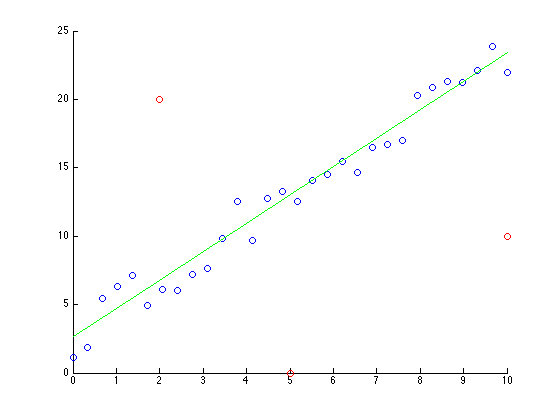
\includegraphics[width=0.5\linewidth]{ransac2d.png}

  \end{center}
  \caption{2D line-fitting using RANSAC.  The resulting line (green) after using RANSAC on 30 inliers (blue) and 3 outliers (red).  Parameters include 100 iterations, 2 samples used per iteration, a distance $\epsilon = 2$ when determining if point is an inlier, and an acceptable probability of error of 1e-9. RANSAC will be described in more detail in later parts.}
  \label{fig:pipeline}
\end{figure*}

\textbf{(B)} Next we compute SIFT features for both images \texttt{seoul1.jpg} and \texttt{seoul2.jpg}.  Figure 2 shows a plot of the matching features and correspondences.\newline

\begin{figure*}[t]
  \begin{center}
    %\fbox{\rule{0pt}{2in} \rule{0.9\linewidth}{0pt}}
    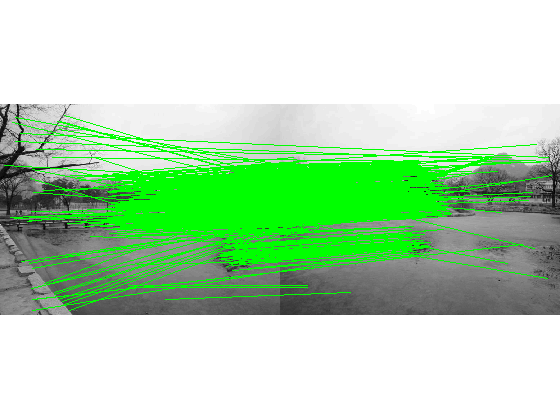
\includegraphics[width=0.75\linewidth, trim= 0pt 80pt 0pt 80pt, clip]{prob1b_1.png}
    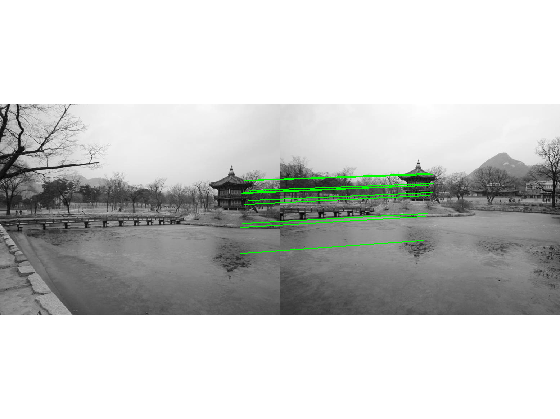
\includegraphics[width=0.75\linewidth, trim= 0pt 80pt 0pt 80pt, clip]{prob1b_2.png}

  \end{center}
  \caption{Resulting matches and correspondences after running SIFT on the overlapping images.  10 matches (bottom) is a more clearly viewed subset from the original 808 matches (top). }
  \label{fig:pipeline}
\end{figure*}

\textbf{(C)} This question pertains to the function \texttt{H = FitHomograohy(x1, x2)}. Given a set of points from two images, we want to compute the homography from the set of points from the overlapped image to the original.  This can be reduced to solving a least squares problem.  We would like to minimize $||Ah = 0||^{2}$, where $Ah=0$ is defined below.\newline
$$
\begin{bmatrix}
x_n & y_n & 1 & 0 & 0 & 0 & -x_{n}'x_{n} & -x_{n}'y_{n} & -x_{n}' \\[0.3em]
0 & 0 & 0 & x_n & y_n & 1 & -y_{n}'x_{n} & -y_{n}'y_{n} & -y_{n}' \\[0.3em]
...
\end{bmatrix}
\begin{bmatrix}
h_{00} \\[0.3em]
... \\[0.3em]
h_{22}
\end{bmatrix}
=
\begin{bmatrix}
0 \\[0.3em]
... \\[0.3em]
0
\end{bmatrix}
$$
\newline
A is a $2n$x$9$ matrix and h is a $9$x$1$ matrix.  The solution is the unit vector of $h$, which is the eigenvector of $A^{T}A$ with the smallest eigenvalue. Normalization is necessary to account for scaling (ensures third component of 3D point is 1).\newline

\textbf{(D)} This question pertains to \texttt{H = TransformRANSAC(x1, x2)}.  To make the algorithm more robust from outliers, the goal is to perform RANSAC to get the best homography H with the least probablity of error.  In addition to the input and output points for the corresponding images, tunable parameters to the algorithm are necessary and shown below.\newline\newline
\texttt{
\textbf{Niter = 10000;}      \%Number of iterations\newline
\textbf{epsilon = 10;}       \%Distance threshold when determining if inlier\newline 
\textbf{P = 4;}              \%Number of samples to use when fitting H to best seen so far\newline
\textbf{acceptableProbFailure = 1e-9;}   \%Acceptable probability of failure\newline
}
\newline
Best results were seen with 10000 iterations and an $\epsilon$ of 10, however, for reasonably quick results, 1000 iterations and an $\epsilon$ of 20 was used (Please refer to below figures for results).  For P, At least 4 sample points is needed to solve the least squares equation.  The acceptable probability of failure was arbitrary.  When running RANSAC, we want to limit the failure rate.  This can be accounted for by performing $P(failure) = (1-G^P)^i$, where $G$ is the percentage of inliers to total points and $i$ is the number of iterations seen thus far.  Please refer to \texttt{TransformRANSAC.m} for a better description/overview of the algorithm.\newline

\textbf{(E)} This question pertains to \texttt{im = MakePanorama(im1, im2, H)}.  The goal is now to produce a panoramic stitch of a H transformed version of im2 onto im1.  To get padding working correctly, I utilized the built-in MATLAB function \texttt{imtransform}.  Therefore, a transformed version of an image can be easily implemented as seen below.\newline\newline
\texttt{
T=maketform('projective',H);\newline
im2t=imtransform(im2,T,'XYScale',1); %Adjust for scaling
}
\newline

\begin{figure*}[h]
  \begin{center}
    %\fbox{\rule{0pt}{2in} \rule{0.9\linewidth}{0pt}}
    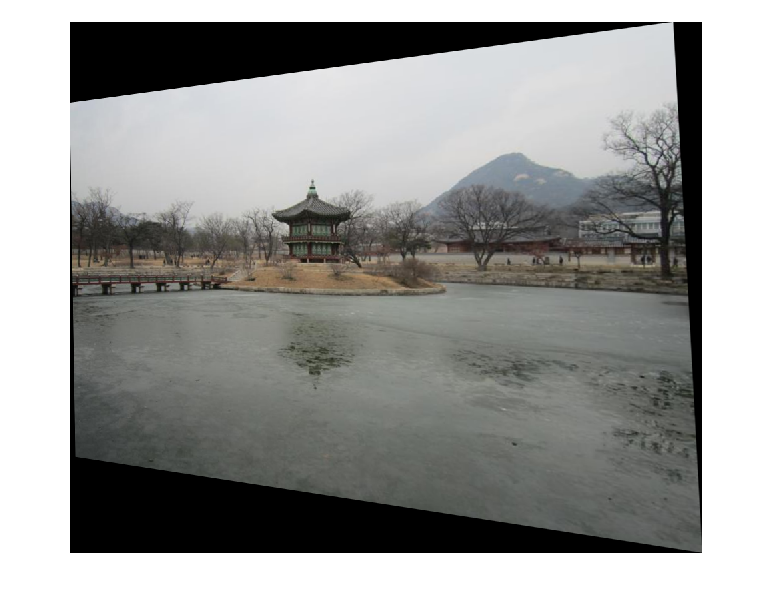
\includegraphics[width=.65\linewidth, trim= 0pt 20pt 0pt 20pt, clip]{im2t.png}

  \end{center}
  \caption{Transformed image of \texttt{seoul2.jpg} after applying H optimized by RANSAC. }
  \label{fig:pipeline}
\end{figure*}

\textbf{(F)} This question pertains to the function \texttt{im = Photomerge(im1, im2)}. This combines the previous parts where an overall panorama is produced given two images.  The first image is used as reference.  The summarized steps to produce the panorama is as follows:

\begin{itemize}
  \item Produce matches/correspondecies by running SIFT
  \item Extract points \texttt{x1,x2} from matches.
  \item Get H: \texttt{H = TransformRANSAC(x2,x1)} (want to transform im2)
  \item Get stitched image: \texttt{im = MakePanorama(im1, im2, H)} 
\end{itemize}

\begin{figure*}[h]
  \begin{center}
    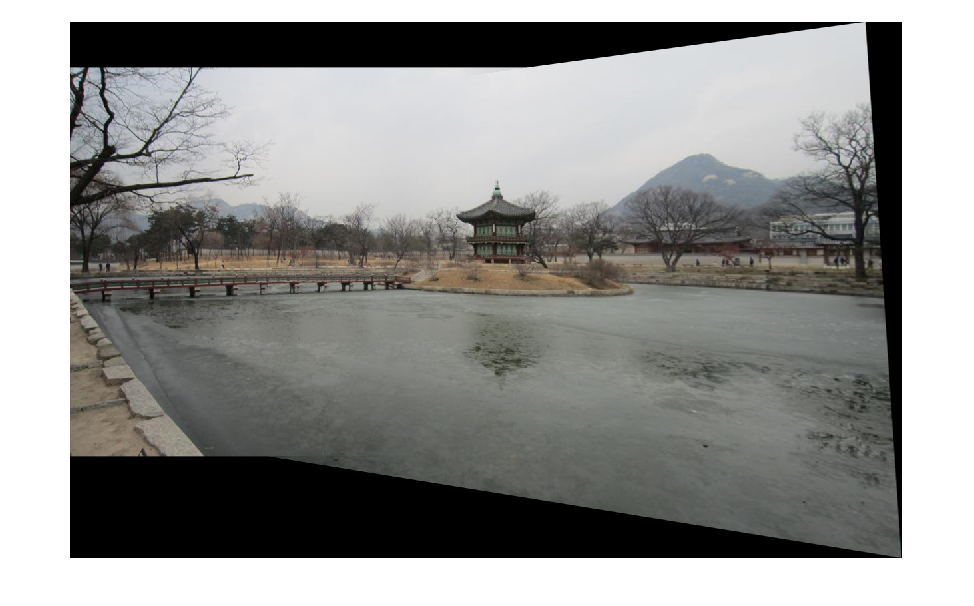
\includegraphics[width=.75\linewidth, trim= 0pt 20pt 0pt 20pt, clip]{pano_2.png}

  \end{center}
  \caption{Results after running \texttt{PhotoMerge.m} on the first two seoul images.  This used $N=1000, \epsilon=20$.}
  \label{fig:pipeline}
\end{figure*}

\textbf{(G)} This question pertains to the function \texttt{im = PanoramaN({im1, im2, ..., imN})}. This function creates a panorama from multiple images and sets the middle image in the list as reference.  Refer to \texttt{PanoramaN.m} for implementation.  Basically, I perform \texttt{PhotoMerge} N-1 times, keeping track which image (left onto right, right onto left) needs to be performed.  Refer to Figure 5 for images $n>2$ resulting panoramas.  It should be noted that when stitching images together, it was necessary to blend pixels as best we could.  It is important that both images are of the same dimension, with added padding if necessary.  When images intersect, take the average of both images.  If they don't intersect, take the value of the valid image.  A summary of choosing/blending pixels is shown below, taking advantage of masking.\newline

$I_{out} = I_{1}(M_{1} \& \sim M_{2}) + I_{2}(M_{2} \& \sim M_{1}) + 
(I_{1}/2 + I_{2}/2)(M_{1} \& M_{2})$

\begin{figure*}[h]
  \begin{center}
    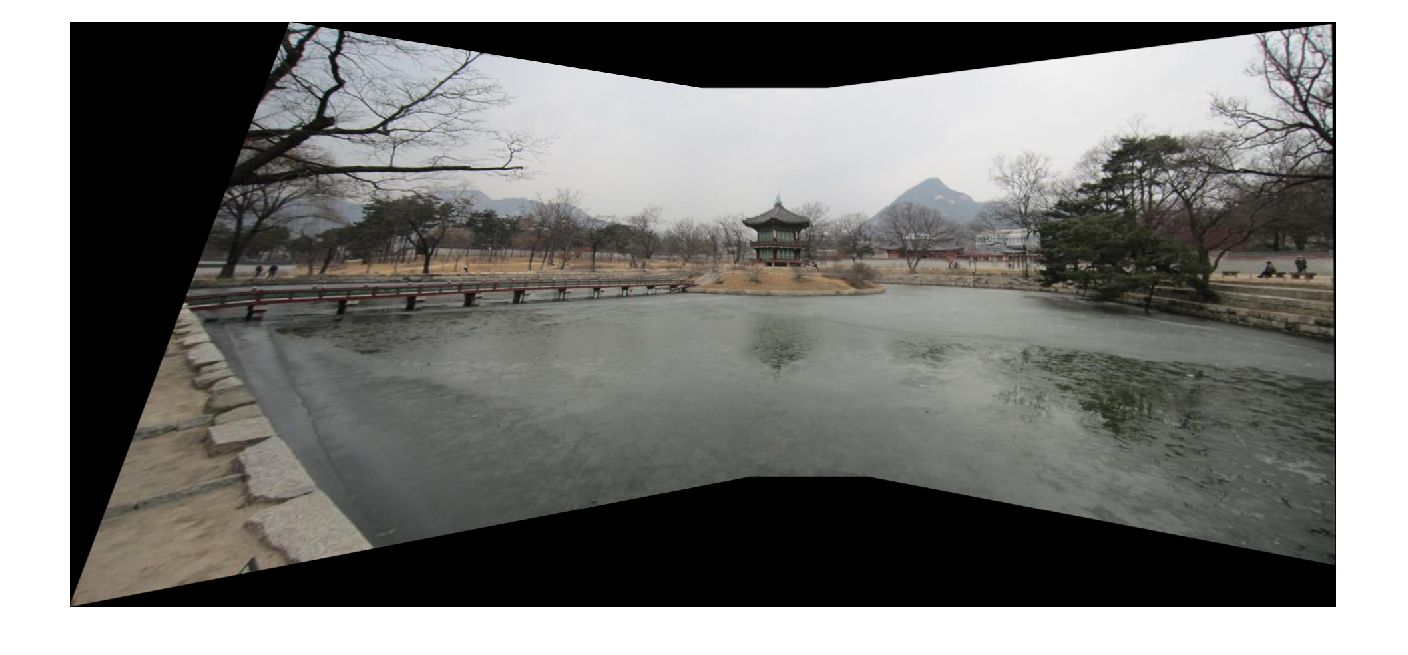
\includegraphics[width=.75\linewidth, trim= 0pt 20pt 0pt 20pt, clip]{pano_3.png}
    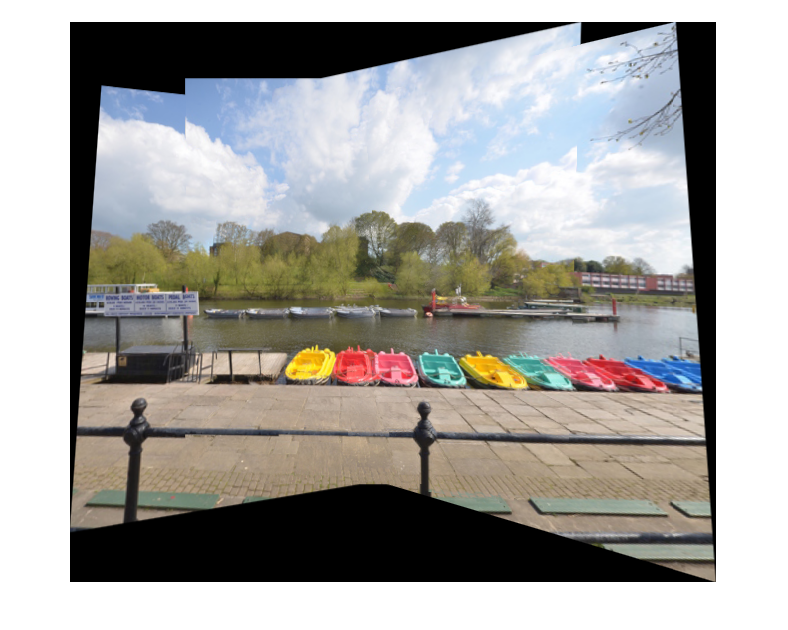
\includegraphics[width=.52\linewidth, trim= 0pt 20pt 0pt 20pt, clip]{pano_4.png}

  \end{center}
  \caption{Results after running \texttt{PanoramaN.m} on the 3 seoul images (top) and the 4 riverbed images (bottom).  They both used used $N=10000, \epsilon=10$. Note: with more images used, stitching and finding inliers relies on the parameters used, therefore, some artifacts may exist.}
\end{figure*}

\textbf{(H)(i)} This question pertains to why a homography suffices for aligning two images.  Let $P_{1} = K[I|t_{1}]$ and $P_{2} = K[R|t_{2}]$ be the corresponding camera matrices. Let $x_{1} = P_{1}X$ and $x_{2} = P_{2}X$. Show that there exists a homography $H$ such that $x_{2} = Hx_{1}$.\newline

\hspace{40pt} $x_{2} = Hx_{1}$\newline
\hangindent5em $P_{2}X = HP_{1}X$\newline
\hangindent5em $K[I|t_{1}]X = HK[R|t_{2}]X$, apply substitutions\newline
\hangindent5em $K[R|t_{2}]^{-1} K[I|t_{1}] X  = HX$, apply inverse rotation matrix\newline
\hangindent5em $ K[R|t_{2}]^{-1} K[I|t_{1}] X X' = H$, where $X'=X^{-1}$ (inverse 3D world point)\newline

This shows that there exists a homography H that does the transformation from $x_{1}$ to $x_{2}$.\newline\newline
\textbf{(H)(ii)} Optional.



\end{document}
